\chapter{Part 2}
%Learning Objectives
%• Embedded control system design using industrial tools
%• Familiarising with a state-of-the-art timing analysis tool from
%INCHRON*
%• INCHRON is a German automotive company which has
%several well-known analysis tools used by companies like
%BMW, AUDI, Daimler etc.


\section{Introduction}
%• Very brief introduction of the overall problem setting (< page
%max)

Analyzing and confirming broad analysis done on paper and in Matlab allows us to confirm the hypothesis made about the behavior of the CAN bus and its specific tasks from Part 1. This analyses is done in Inchron, which allows us to explore the real-time behavior of this embedded system in full detail. Some exploration on how the system should work has already been done in Part 1, \color{red} Add Table reference to periods and priorities \color{black}, this is used here by feeding the settings of the embedded system to the tool. The settings included is the hierarchy of the Processing Units (PUs) and their tasks which each have different periods, execution time and priority. The tree view, Figure \ref{fig:treeCAN}, shows the details of the hierarchy from the Inchron's perspective.

\begin{figure}[h!]
	\begin{center}
		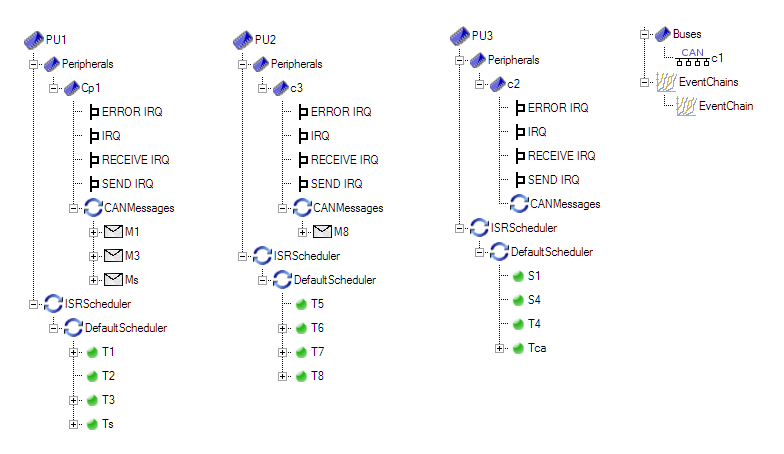
\includegraphics[width=0.75\linewidth]{img/treeCAN}
		\caption{This shows the coarse grain hierarchy of the system ported into Inchron for verification and simulation of the real time components of our embedded system.}
		\label{fig:treeCAN}
	\end{center}
\end{figure}




\section{Response Time analysis}

\subsection{Response time analysis per processing unit}
%• Response time analysis per processing unit (plots and brief description)

For this analysis all details have to be imported to Inchron as stated earlier. Now paying special attention to the messages which transfer the packets between controllers which make a full system. 

When validating and simulating the model with the settings mentioned in Part 1 and Figure \ref{fig:treeCAN} and \ref{fig:msgCAN} we can observer the response times for each task when inserting the Worst Case Execution Time into the tool. Next each processing unit and their Worst Case Response Time (WCRT) will be investigated and then compared to the Matlab model (Response Time analysis). The resulting figures were obtained after several tries with various settings until the correct configuration of the tool was found, e.g. setting the schedule as preemptive was not set as it was not found in the first try.

\subsubsection{PU1}

For PU1 a fixed preemptive priority scheme with four tasks T1,T2,T3 and Ts. Now when validating the model, Figure \ref{fig:pu1rt} is obtained showing the results and they are compared to the Matlab response times in Table \ref{tab:pu12}.

\begin{figure}[h!]
	\begin{center}
		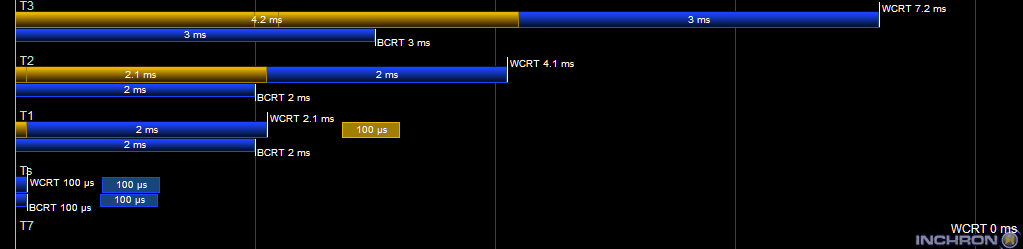
\includegraphics[width=\linewidth]{img/pu1-response-time}
		\caption{Showing the WCRT analysis for PU1. The Results can be read from each horizontal bar.}
		\label{fig:pu1rt}
	\end{center}
\end{figure}

\subsubsection{PU2}
Now PU2, has the same sheme as PU1, fixed preemptive priority, with four tasks T5,T6,T7 and T8. Now when validating the model, Figure \ref{fig:pu2rt} is obtained showing the results and they are compared to the Matlab response times in Table \ref{tab:pu12}.

\begin{figure}[h!]
	\begin{center}
		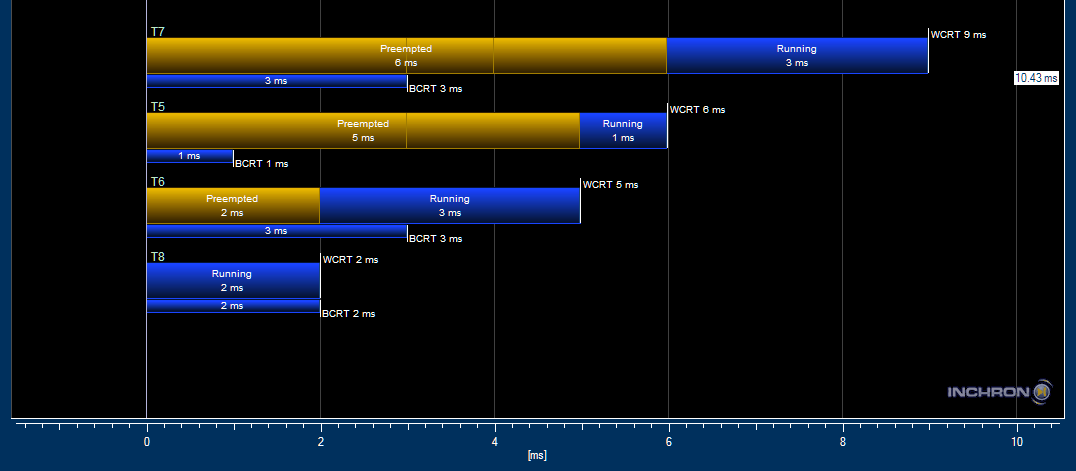
\includegraphics[width=\linewidth]{img/pu2-response-time}
		\caption{Showing the WCRT analysis for PU2. The Results can be read from each horizontal bar.}
		\label{fig:pu2rt}
	\end{center}
\end{figure}

\subsubsection{PU3}

Allthough PU3 has a time division multiplexing (TDM) its tasks will still be analyzed here, shown in Figure \ref{fig:pu3rt}. It is important to state that T4 is not a real-time task as it is sending a message \textit{out to the blue} but $T_{ca}$ is an important task, actuating on the sensor value and completing the sensor to actuator delay.

\begin{figure}[h!]
	\begin{center}
		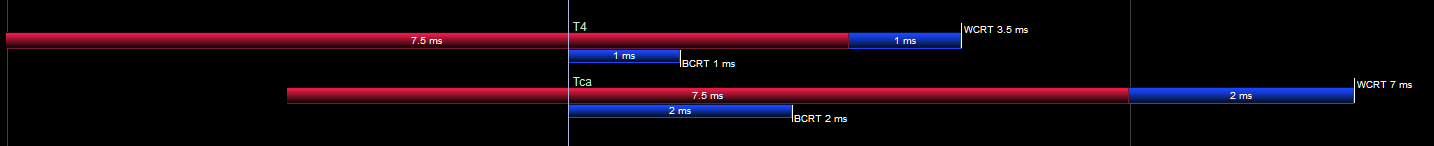
\includegraphics[width=\linewidth]{img/pu3-response-time}
		\caption{Showing the WCRT analysis for PU3 (TDM). The Results can be read from each horizontal bar}
		\label{fig:pu3rt}
	\end{center}
\end{figure}


\begin{table}[htbp!]
	\centering
	\caption{By running the Matlab script ResponsetimeAnylsis\_FPP.m with the different parameters given for PU1 and PU2 these response times are obtained. These files are then delivered as PU1.m and PU2.m}
	\begin{tabular}{rrrrc}
		& & & & \\
		\toprule
		PU1     & $T_1$    & $T_2$    & $T_3$    & $T_4$  $(T_s)$ \\
		\midrule
		Matlab (ms)      & 0.1     & 2.1     & 4.1     & 7.2 \\
		Inchron (ms)	& 0.1     & 2.1     & 4.1     & 7.2 \\
		
		& & & & \\
		\toprule
		PU2     & $T_5$    & $T_6$    & $T_7$    & $T_8$ \\
		\midrule
		Matlab (ms)      & 6       & 3       & 9       & 5 \\
		Inchron (ms)	 & 6       & 3       & 9       & 5 \\
		
	\end{tabular}%
	\label{tab:pu12}%
\end{table}%


\pagebreak
\subsection{ Response time analysis for the CAN bus messages}
%• Response time analysis for the CAN bus messages

PU1 and PU2 are the only units within the system that are sending messages, shown for clarity in Figure \ref{fig:msgCAN}, but PU3 contains the computing and actuating task which will receive the $m_s$ message and mark the end of the sensor to actuator delay. 

\begin{figure}[h!]
	\begin{center}
		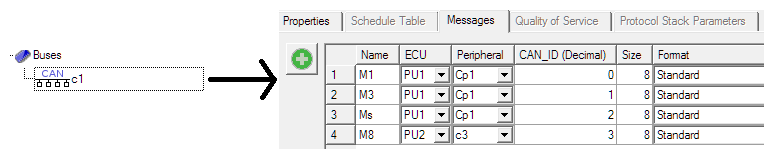
\includegraphics[width=\linewidth]{img/msgCAN}
		\caption{All can messages in the system, indicating PU source, individual CAN id and message size in bytes}
		\label{fig:msgCAN}
	\end{center}
\end{figure}

\begin{figure}[h!]
	\begin{center}
		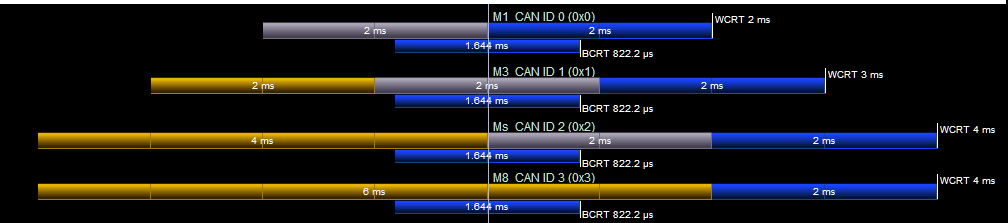
\includegraphics[width=\linewidth]{img/messagesCANtimings}
		\caption{Showing the WCRT analysis for the CAN messages. The Results can be read from each horizontal bar and is compared in Table \ref{tab:can-rts}.}
		\label{fig:msgCANtiming}
	\end{center}
\end{figure}

\begin{table}[htbp!]
	\centering
	\caption{CAN messages of the system compared from the Inchron tool suite and Matlab. Showing identical results}
	\begin{tabular}{rrrrr}
		\toprule
		CAN     & $m_2$   & $m_1$   & $m_3$   & $m_8$ \\
		\midrule
		Matlab ms & 2       & 3       & 4       & 4 \\
		Inchron & 2       & 3       & 4       & 4 \\
		\bottomrule
	\end{tabular}%
	\label{tab:can-rts}%
\end{table}%


\pagebreak

\section{Optimization for sensor-to-actuator delay}
%• Optimisation for sensor-to-actuator delay (include troubleshooting)

Now optimizing the sensor-to-actuator delay requires running the CrhonOpt tool within Inchron and setting up objectives for the real time requirements. That will be set to target: event-chain, which is set to be smaller or equal to 5ms.

The initial priorities were selected according to period and execution time, shown in Figure \ref{fig:inchronprios} on the left, but when running the simulation to enhance the sensor to actuator delay, the tool changed the priorities in PU2, shown in Figure \ref{fig:inchronprios} on the right. This showed to be an improvement although this did not change the sensor to actuator delay.

\begin{figure}[h!]
	\begin{center}
		\begin{tabular}{cc}
		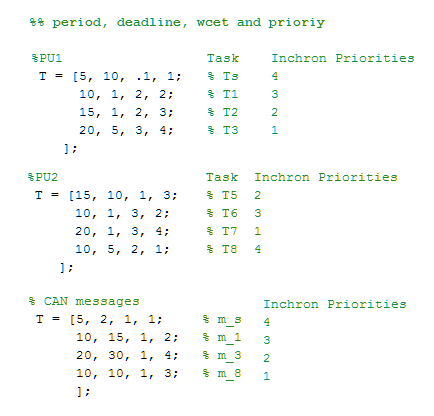
\includegraphics[width=0.5\linewidth]{img/inchron-prios} & 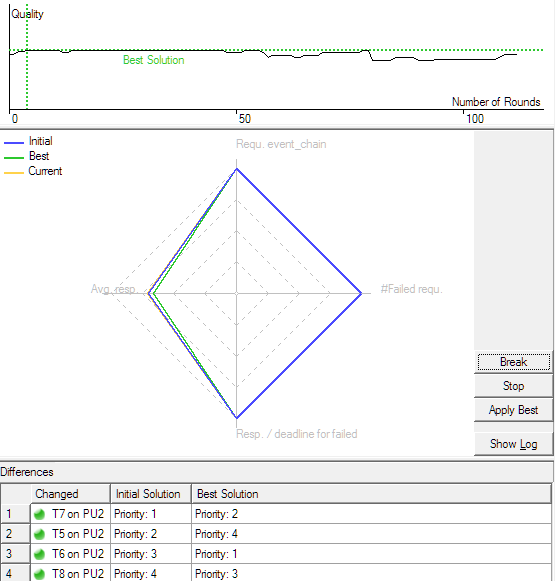
\includegraphics[width=0.5\linewidth]{img/optimized}	\\
		\end{tabular}
		\caption{On the left, initial priorities used in the Matlab script and on the right the ChronOPT optimization of these parameters. }
		\label{fig:inchronprios}
	\end{center}
\end{figure}




\section{System model}
%• System model derivation, design space exploration and controller
%parameter design

\section{Design decision}
%• Your design decision and justification.



\section{Results}
%• Results
%− Response time analysis

Firstly: Response time analysis\\
Secondly: Plots from chronVIEW (before and after optimization)\\
Last: Control system input and output

\section{Conclusions}